\section{Data Ownership} 
\label{section:DataOwnership}

% General overview defining data as an asset, actors in data economy, and how SDL can expand 

In this section, we will define data ownership, explain why defining data as an asset is tricky, and establish the flow of value in the current data economy.

\subsection{Ownership}


% How can individuals control / own their data
The Snickerdoodle Protocol aims to shift the balance of power within the existing data economy by providing individuals greater control of their data. 
To do so, we must first understand the value within the existing data economy and what it means to control and own data. 

\begin{definition}
\label{definition:DataOwnership}
Data Ownership: If an individual can exclusively control and manage the collection, storage, and usage of an attribute of their data corpus in a secure 
and private manner, then it can be said that they own that particular data attribute.
\end{definition}

% The goal of this protocol is to maintain the value in the current data economy while flipping the power structure on its head by giving individuals control of the data they generate. This is consistent with the trend we see in modern legislation (CONTINUE TO GIVE CONTEXT).

Ownership of data is a difficult concept to define. Unlike physical resources, data can be copied indefinitely, is generated constantly, and generally requires 
technical expertise and extensive cyber infrastructure for collection and value extraction. Because of these properties, the safety of data is crucial to data ownership and 
makes regulating the use of data inherently difficult.

To illustrate these properties, let us use the example of Alice: a customer shopping at a grocery store. By simply being at the store, Alice has generated data about 
which store she shopped at and when. When she checks out, she generates data about what products she has bought and what payment method she used. When she leaves, 
she generates data about how long she has been in the store. All of this data may have value, and several actors may be collecting it. The store may be collecting 
this data through surveillance or loyalty programs. Her phone may have software collecting her location data. Her credit card company may be tracking her spending 
habits. In the existing data economy, these entities performing the collection have total sovereignty of these data attributes. They may analyze this data for targeted 
advertising, conduct market research, or sell it to other parties. In addition, companies collecting this data may take all of these actions with varying standards 
of privacy, security, or anonymity for Alice. Alice is not likely to have knowledge about what data attributes were collected, who collected it, who has access to it, or how 
the data is used. She is also not compensated for the value that is extracted from this data, even though she is the entity from whom originated it.

In the above example, the concerns around collection and privacy are immediately apparent, but this example also brings into question what it means to own data. 
In Alice's case, her data is being collected by third parties who may sell or exchange it with other parties. Due to the infinite duplicability of digital data, any 
such exchange results in both parties possessing the data. In this case, who actually owns the data? Is it the party that collected it? Is it collectively owned by 
all parties that are currently storing it? Or is it owned by the party that originated it (Alice)? In the existing model, data is owned by the entities that store it, 
and may be legally attributable to the entity that collected it (CITE). According to definition \ref{definition:DataOwnership}, Alice would have control of her data 
if she knew what aspects about her were being observed, had control over who was able to access the information, and the infrastructure used to collect, store, and 
access the data did so safely.

% Feel like with other sections this has become redundant
% I've like the ideas in here so have commented it out for now. We can un-comment if we delete other sections that discuss this ()
%
% In the case of data, privacy and security are critically important since compromised data is no longer self-sovereign. If another party has gained access to the data, it is virtually impossible to maintain data ownership as exclusivity has been lost. This is why the Snickerdoodle Protocol aims to provide privacy and security by exchanging data insights rather than the data itself. Additionally, data management should be easy for the user.

\subsection{Data as an Asset}
% Data has value and can be treated as an asset. How is it different/similar to traditional assets
% https://money.cnn.com/news/newsfeeds/articles/stocktwits/pointsandfigures_9937.html?iid=EL#:~:text=Commodities%20are%20assets%2C%20but%20unlike,can%20derive%20out%20of%20them.
In an information economy, data is the most fundamental commodity there is. To understand the individualized data economy, we must highlight the difference between assets 
and commodities. While commodities are an asset class, they have unique properties. Unlike most other asset classes, commodities are traded at high volume. While it is 
possible to purchase small volumes of commodities, they are often illiquid due to the markets operating at high volumes. While fractional vehicles like ETFs do exist, 
these are fundamentally not equivalent, as they represent nothing more than a symbolic debt obligation and not the resource itself. For example, it is possible to buy 
an individual gallon of oil but much harder to sell it as the markets do not trade oil by the gallon. Conversely, it is much easier to sell a thousand barrels of the 
same oil since the commodities markets trade at these quantities regularly. In much the same way, individual data is not valuable in today's data economy and is almost 
exclusively traded in the aggregate.

There are cases in which individualized markets have developed around commodities. For example, in the wake of the 2008 financial crisis, consumers rushed to purchase gold as trust in financial assets, currencies, and markets plummeted. Nations and banks often trade in gold in large quantities, and as a result, gold markets trade-in units ranging from the thousands to the millions. To facilitate the liquidity of consumer gold, several gold purchasing operations have sprung up to provide liquidity to the individual and aggregate gold for commodities markets. Because of the non-triviality of data ownership (see below), this infrastructure has yet to be created for data. This is what the Snickerdoodle protocol aims to enable.


\subsubsection{Utility of Data}
% What can we do with data

% What is the value of data 
%.      How can people get value
%       How can businesses get value

Data provides so much utility in the twenty-first century and has revolutionized every industry from supply chain to medicine, biotech, sports, and self-driving cars. Some of this involves insane computing, such as using machine learning to generate human faces and stories, to less complex tasks like finding the quickest route home. There is also a dark side to this, as all this data allows for complex and automated ways to track people. (MORE CITATIONS). 

We find that the utility of data comes from the ability the analyze data to generate $\mathit{insights}$. These insights help us understand the world and allow us to make more informed actions. E.g., Google uses my search history to learn what I like and give a relevant ad. A self-driving car analyzes data from its sensors to learn that the traffic light turned red and it should stop.

\subsubsection{An individual's role in the data economy} 
%TODO moving this to the top bc I think it'll help if flow better -- not sure where on the top it fits the best
% What is the role of an individual right now?
% Looking at the flow how can an individual's role be expanded
The problem with the current data economy is that the individual generating the data doesn't have control over how their data is being used and isn't being properly compensated for their role in the data economy. Different governments recognize the need to give users control, such as the GDPR and CCPA (CITE THINGS + maybe more info). While the data economy is said to be valued around XXX at the time of writing (CITE), individuals aren't getting their fair share of this pie. (NEED MORE CITATIONS -- maybe Kara Swisher cheap date, also need harder sources). 
\newline
\newline
Another problem is that the lack of ownership and control of data leads to ways for governments to get around surveillance laws. Instead of getting a warrant to view individual data, governments can buy the data from data brokers (CITE). This creates an opaque way for governments to spy on individuals. For example, the US government's ICE agency created an extensive database through publicly available information and data brokers that allow them to track everyone in the US without a warrant (CITE). 


% Due to how tricky it is to define data ownership, our protocol focuses on allowing users to control data they they generate. Specifically we want to enable a protocol that gives users to safely managed how their data is collected, stored, and shared. Additionally, parties that are interested in subscribing to individual's data can do so without compromising the safety of that data. The protocol should also maintain the authenticity and interoperability of data to ensure that the data being process is valid and usable.

%        How technically they can do this -- Introduce data wallet

%  Data asset life cycle
% collect/store/share/manage/own

\subsubsection{Properties of Data}
% trying italic special sections not sure if it works
It's worth highlighting that when data is treated as an asset, the value of the data asset can depend on the properties of that data. The $\mathit{utility}$ of the insights that data can provide will dictate how valuable the data is. $\mathit{Privacy}$ of the data is vital in creating value out of data. If data isn't private, there's no scarcity of data, and the asset is worth less. Worse, the lack of privacy incentives enables mass surveillance.
Similarly, $\mathit{security}$ is deeply tied to the value of data as an asset. Data that isn't secure can easily be stolen or can be rendered unusable. 
Data should be $\mathit{interoperable}$, so it can be used across many platforms. If my data is in a proprietary format or can't be moved outside of a particular system, there's less demand for the data. 
There also needs to be ways to gauge the $\mathit{authenticity}$ of the data. If the data can easily be faked, then the data is worth less.


% good points I had to delete:
% hard to maintain privacy when it is shared
% manage the deletion of data
% maintain forward and backward secrecy
% security in all forms (storage and transit)
% needs to be easy to do maintain good security practices and patch bugs
% Integrate with other providers and identity management solutions
% Authenticity and Privacy are sometimes at odds -- I want Cali DMV to validate I am over 21 but if they vouch for me other people know I am a Cali resident


% When turning data into an asset, there are important properties that need to be considered. Who gets to see the asset (privacy), how secure is the asset(security), how easy it is to get value out of the asset (interoperability), and is the asset legitimate (authenticity).  


\subsection{Flow of Data and Value in the Data Economy}
\label{section:Actors}
% TODO should we define verified and unverified data?
% Who is involved in the data economy
%.    Break down into personas
%.    Break down how data flows

The data economy is a complex system that collects data on individuals, shares that data with other actors, and runs analysis on that data. This flow is necessary to extract value from data. The people generating the data don't necessarily have a good way to take advantage of their data, and those interested in the data don't generate it. This dynamic is at the heart of the data economy. One group generates the data, and the other wants to gain insight from that data. The rest of the actors exist to provide infrastructure to support that dynamic. This flow can be seen in figure \ref{fig:DataActors}.


\subsubsection{Actors}
We define the generator of the data as the $\mathit{owner}$ and the actor who is interested in the data as the $\mathit{subscriber}$. Being the entity that creates the data, the owner should have ownership rights and thus control how their data is used. The subscriber is interested in gaining temporary access to that data and running an $\mathit{application}$ on a large amount of data to learn insights and use those insights to take specific actions. It's worth highlighting that, in our definition, the subscriber is only interested in the utility of the data, not the data itself.


Other actors in the economy provide the infrastructure. $\mathit{Collectors}$ are the actors who monitor and collect data on owners. $\mathit{Custodians}$ store that data. Because the utility of data increases when combined with other data, the $\mathit{aggregator}$ aggregates data from different custodians and makes it easy to run applications to generate insights.


Subscribers pay for the utility, and that payment flows back down through the economy. Also, note that the same entity can play multiple roles. E.g. Google is a collector, custodian, aggregator, application, and subscriber for ads on web searches. Subscribers pay Google to run an application that analyzes people and gives ads to those they think are interested in the subscriber's product. Data owners are the people using Google search. They are getting back a free online search and pay Google by seeing ads and allowing Google to control the data.


For this to be a self-sovereign data economy, the data owner must own their data and thus control how it is used. The owner must be able to easily manage the collection, storage, aggregation, and applications that run on their data. Additionally, payment must be distributed equitably to the parties in this economy such that the owner gets their fair share and all the actors have an incentive to behave.

TODO UPDATE FIGUTE TO SHOW ACTORS AND SNICKERDOODLE ACTORS
\begin{figure*}[!htbp] 
    \centering
    % \textbf{a.}
    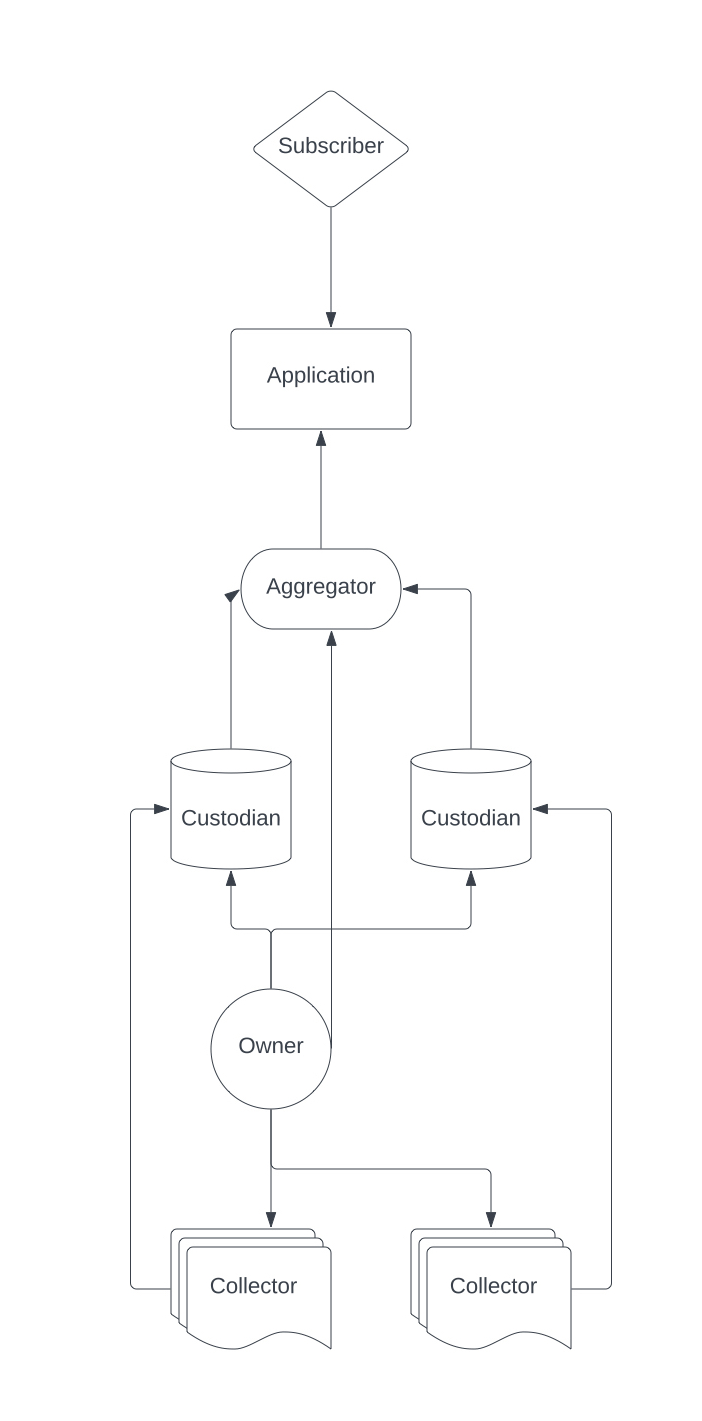
\includegraphics[width=170]{images/persona_strucutre.jpg}
    \caption{The flow of data in the data economy. The data is generated by the owner and flows from collectors to custodians to aggregators to applications and finally to the subscriber. The subscriber pays money that trickles back through the system. In order for the owner to actually have ownership of their data they must be able to manage the collector, custodian, and aggregator of their data.}
    \label{fig:DataActors}
\end{figure*}



\subsubsection{Actors in the Snickerdoodle Protocol}
% For our version 1 how are we going to break down the actors/personas
%     Individual's / end users
%.    Businesses
%     DAO
%.    SDL
We will simplify the actors for the initial version of the Snickerdoodle Protocol. The users of the protocol are data owners who will collect, store, and manage their data from a $\mathit{data wallet}$ (for more on data wallet, see \ref{section:DataWallet}). The data wallet will allow people to consent to aggregation and allow certain applications to run on their data by minting a non-transferable consent NFT (to learn more about the on-chain aggregation\&consent architecture and the applications, see sections \ref{section:Contracts} and \ref{section:SDQL} respectively). Lastly, consenting data wallets will send the resulting insights to an ingestion provider, which will allow businesses to see the insights they have paid for (see \ref{section:InsightService}). 


For implementation details check out section \ref{section:Implementation} and for ways we'll expand the protocol in the future check out section \ref{section:Future}.
